\documentclass{article}

\usepackage{amsmath, amsfonts, amssymb}
\usepackage{enumerate}
\usepackage{graphicx}
\usepackage{wrapfig}
\usepackage{listings}

\lstset{language=Matlab, tabsize=2, showstringspaces=false, breaklines = true}

\newcommand{\R}{\mathbb{R}}

\title{Homework 2}
\author{Matthew Dupraz}

\begin{document}

\maketitle

\section*{Section 1: Theory}

Let $f: \R \to \R$ be twice continuously differentiable in a 
neighbourhood of $x\in \R$

\begin{enumerate}[(a)]
   \item
      The Taylor remainder theorem tells us that for all $h > 0$,
      there exists some $\eta \in [0, 1]$ such that
      \begin{equation*}
         f(x + h) = f(x) + f'(x)h + \frac{1}{2}f''(x + \eta h)h^2
      \end{equation*}
      Hence
      \begin{equation*}
         \left|\frac{f(x + h) - f(x)}{h} - f'(x)\right| =
         \frac{1}{2}|f''(x + \eta h)|h
      \end{equation*}
      Since $f''$ is continous, for all $\epsilon > 0$, there
      exists some $\delta > 0$ such that 
      $\forall h \in B(0, \delta)$,
      \begin{equation*}
         \left|\frac{1}{2}f''(x + \eta h) - \frac{1}{2}f''(x)\right| < \epsilon
      \end{equation*}
      So for all $h \in (0, \delta)$,
      \begin{equation*}
         \left|\frac{f(x+h) - f(x)}{h} - f'(x)\right| \leq 
         \left(\frac{1}{2}|f''(x)| + \epsilon\right)h
      \end{equation*}
      So if we take the limit $\epsilon \to 0$, we get
      $\tilde{C} = \frac{1}{2}|f''(x)|$
   \item
      The difference between the real and computed finite difference quotient
      is:
      
      \begin{align*}
         \Bigg|\frac{f(x+h) - f(x)}{h} &-
         \frac{f(x+h)(1 + \delta_1) - f(x)(1 + \delta_2)}{h}\Bigg| = \\
         &= \left|\frac{f(x+h)\delta_1 - f(x)\delta_2}{h}\right|\\
         &\leq u\frac{|f(x+h)|+|f(x)|}{h}
      \end{align*}

      So $c = |f(x + h)| + |f(x)|$ and if we take the limit
      $h \to 0$, we get $\tilde{c} = 2|f(x)|$
   \item 
      The difference between the computed finite difference quotient and the 
      derivative can be approximately bounded by:
      \begin{align*}
         &\Bigg|\frac{f(x+h)(1 + \delta_1) - f(x)(1 + \delta_2)}{h}
         - f'(x)\Bigg| \leq \\
         &\leq 
         \Bigg|\frac{f(x+h)(1 + \delta_1) - f(x)(1 + \delta_2)}{h} -
         \frac{f(x+h) - f(x)}{h}\Bigg| \\
         &~~~+ \Bigg|\frac{f(x+h) - f(x)}{h} - f'(x)\Bigg| \\
         &\lessapprox 2|f(x)|\frac{u}{h} + \frac{1}{2}|f''(x)|h
      \end{align*}
   \item
      Hence we can approximate the upper bound of the error with the following function:
      \begin{equation}
         err(h) = 2|f(x)|\frac{u}{h} + \frac{1}{2}|f''(x)|h
      \end{equation}
      We can find the minimum by computing the derivative:
      \begin{equation}
         err'(h) = -2|f(x)|\frac{u}{h^2} + \frac{1}{2}|f''(x)|
      \end{equation}
      So if $f''(x) \neq 0$, we get that
      \begin{equation}
         err'(h) = 0 \iff h^2 = 4u\left|\frac{f(x)}{f''(x)}\right|
      \end{equation}
      And so in theory we get the smallest error when
      $h_{min} = 2\sqrt{u\left|\frac{f(x)}{f''(x)}\right|}$.
      If $f''(x) = 0$, the function $err$ does not admit a minimum.
      For the specific case of $f = \exp$, $x = 1$ and
      $u = \frac{1}{2}2^{1 - 53}$ (matlab uses double precision floating
      point numbers), we get $h \approx 2.1 \times 10^{-8}$.
      Indeed, when we graph the real and theoretical errors against $h$ on a single plot, we
      get the following figure:\\
      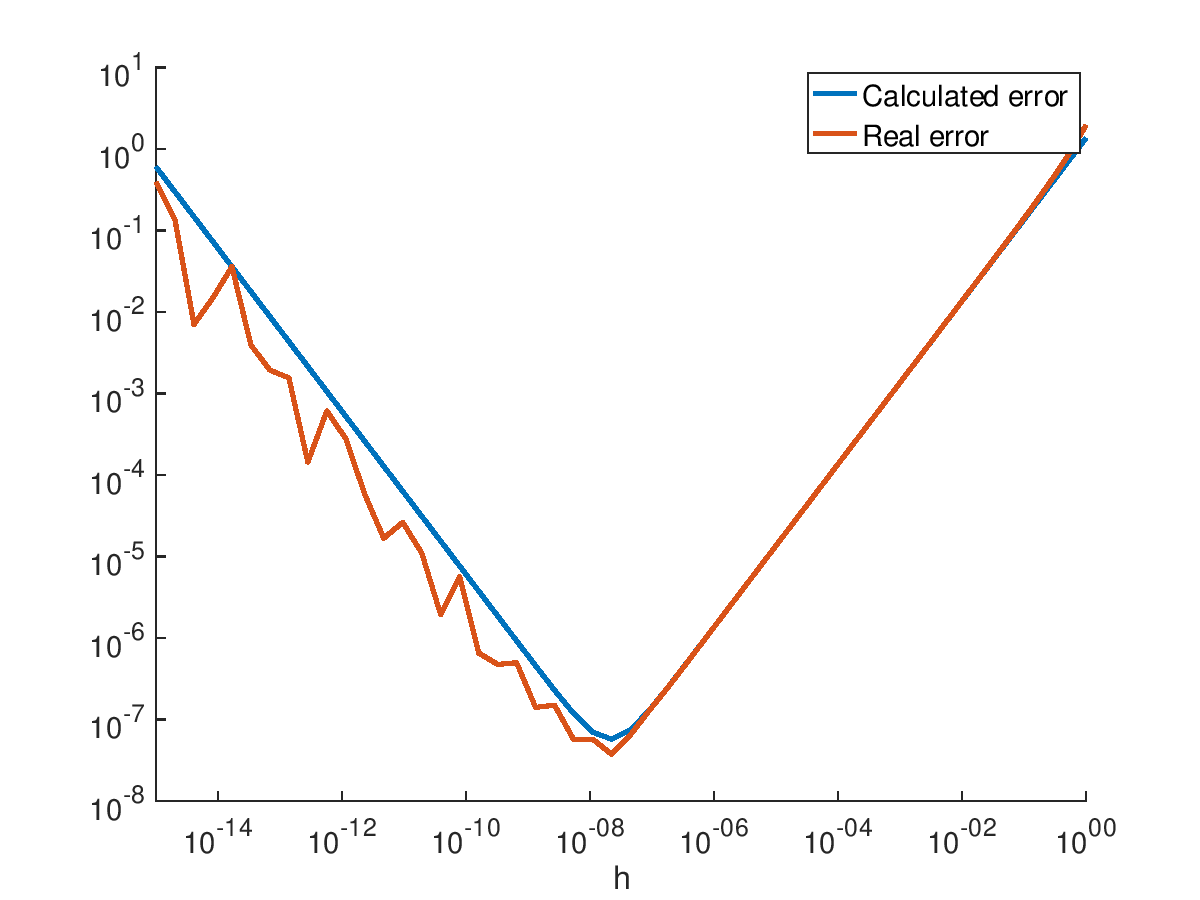
\includegraphics[width=0.6\textwidth]{figure}

      The red curve is the real error and the blue one is the
      theoretical approximate upper bound.
      So we see the function we found approximates the real error
      quite closely.
\end{enumerate}

\subsection*{Code for plotting the errors}

\begin{verbatim}
% beta = 2, t = 53
u = 2^(-53);

err = @(h) 2*exp(1)*u./h + 1/2*exp(1).*h;
real_err = @(h) abs((exp(1+h) - exp(1))./h - exp(1));

xs = logspace(-15, 0);

% Plotting values
hold on;
loglog(xs, err(xs), 'LineWidth', 2);
loglog(xs, real_err(xs), 'LineWidth', 2);

% Configuring axes style
xticks(10.^[-14:2:0])
xlabel('h');
set(gca, 'FontSize', 14);

% Setting up the legend
lgd = legend('Calculated error', 'Real error');
set(lgd, 'FontSize', 14);
\end{verbatim}

\section*{Section 2: Matlab}

The values calculated for the answers of this exercise are shown below:

\begin{verbatim}
--------------------
Quadratic 1: x^2 + 2.5x + 1
Calculated roots to 1: x+ = -0.5, x- = -2
Real roots to 1: x+ = -0.5, x- = -2
Relative errors to 1: x+ -> 0, x- -> 0
Evaluation of 1 at computed roots: P(x+) = 0, P(x-) = 0
Recovered bad root of 1 from good root: -0.5
Evaluation of 1 at revovered bad root: 0
--------------------
Quadratic 2: x^2 + -10000000000x + 1
Calculated roots to 2: x+ = 10000000000, x- = 0
Real roots to 2: x+ = 10000000000, x- = 1e-10
Relative errors to 2: x+ -> 0, x- -> 1
Evaluation of 2 at computed roots: P(x+) = 0, P(x-) = 1
Recovered bad root of 2 from good root: 1e-10
Evaluation of 2 at revovered bad root: 1e-20
--------------------
Quadratic 3: x^2 + 1073741824x + 1
Calculated roots to 3: x+ = 0, x- = -1073741824
Real roots to 3: x+ = -9.31323e-10, x- = -1073741824
Relative errors to 3: x+ -> 1, x- -> 0
Evaluation of 3 at computed roots: P(x+) = 1, P(x-) = 0
Recovered bad root of 3 from good root: -9.31323e-10
Evaluation of 3 at revovered bad root: 8.67362e-19
--------------------
\end{verbatim}

We see that already from the get go the value of $p$ was truncated
in both the second and third quadratic, because Matlab uses double
floating point precision. For example in the third quadratic,
since $t = 53$, the
value of $p$ would have to be represented in the following way:

\begin{equation*}
   p = 2^{30} + 2^{-30} = 2^{31 - 53}(2^{52} + 2^{-8})
\end{equation*}

Since $2^{52} + 2^{-8}$ is not an integer, $p$ is not representable
in the double floating point system.
The value of $p$ in the second quadratic is not precise for the
same reason.

Now the reason why the computed roots differ to real roots is also
due to rounding error during the computation. If we look at the
code below, it might happen that $-p/2$ and $d$ have a difference
that is proportionally much smaller than their magnitude.
More specifically, the difference of the computed values of
$-p/2$ and $d$ is

\begin{equation*}
   -p/2(1 + \delta_1) - d(1 + \delta_2), ~~|\delta_1|,|\delta_2| < u
\end{equation*}

and so the error we get in the calculation is
$-p/2\times\delta_1 - d\times\delta_2$, which in worst case is
$(|p/2| + |d|)u$. This error could be relatively large compared to
the real value of $-p/2 - d$. In the case of our inputs the
calculated roots were often rounded to $0$. This is because the
computed value of $-p/2$ and $d$ were rounded to the same value,
this could happen if the distance between the two numbers was
smaller than the least distance between two consecutive
double precision floating point numbers of that magnitude,
which is $2^{-1}\epsilon_M|p/2|$ in this case. That's why
the relative error is $1$ is those cases. The explanation was for
the lack of precision in $x_2 = x_-$,
but for $x_1 = x_+$ it goes essentially
along the same lines.

Now since the error I described happens when the two numbers are
close together, it is clear that if $p$ is positive, then the bad
root will be $x_+$ and if $p$ is negative, the bad root will be
$x_-$. The results we got in the output above clearly reflect this.
We recovered the bad roots from the good ones using the formula
$x_{bad} = q / x_{good}$ and we notice the roots were accurately
recovered, this is because the relative error between the real and
computed value of $x_{good}$ is small and so will be the error
in the quotient.

\subsection*{Code from roots2.m}

\begin{verbatim}
function [x1, x2]=roots2(p, q)
   d = sqrt(p^2/4 - q);
   x1 = -p/2 + d;
   x2 = -p/2 - d;
\end{verbatim}

\subsection*{Code from main.m}

\begin{verbatim}
% Values of p and q for the three polynomials
ps(1) = 2.5;
qs(1) = 1;
ps(2) = -10000000000.0000000001;
qs(2) = 1;
ps(3) = 2^30 + 2^(-30);
qs(3) = 1;

% Calculating roots of the three polynomials
for i=1:3
   [xs1(i), xs2(i)] = roots2(ps(i), qs(i));
end

% Real roots of the three polynomials
rxs1(1) = -0.5;
rxs2(1) = -2;
rxs1(2) = 10^10;
rxs2(2) = 10^(-10);
rxs1(3) = -2^(-30);
rxs2(3) = -2^30;

% Calculating the errors between
% the calculated and real roots
rel_err = @(x, rx) abs(rx - x)./abs(rx);

errs1 = rel_err(xs1, rxs1);
errs2 = rel_err(xs2, rxs2);

% Evaluating the polynomials at the calculated roots
evs1 = qs + ps.*xs1 + xs1.^2;
evs2 = qs + ps.*xs2 + xs2.^2;

% The bad root is smaller in magnitude
for i=1:3
   if (abs(xs1(i)) >= abs(xs2(i)))
      recov(i) = qs(i)/xs1(i);
   else 
      recov(i) = qs(i)/xs2(i);
   end
end

% Evualuationg polynomial at x_bad
ev_recov = qs + ps.*recov + recov.^2;

% Displaying everything in a readable manner
disp('--------------------')
for i=1:3
   str = sprintf('Quadratic %i: x^2 + %dx + %d', ...
      i, ps(i), qs(i));
   disp(str);

   str = sprintf('Calculated roots to %i: x+ = %d, x- = %d', ...
      i, xs1(i), xs2(i));
   disp(str);

   str = sprintf('Real roots to %i: x+ = %d, x- = %d', ...
      i, rxs1(i), rxs2(i));
   disp(str);

   str = sprintf('Relative errors to %i: x+ -> %d, x- -> %d', ...
      i, errs1(i), errs2(i));
   disp(str);

   str = sprintf(...
      'Evaluation of %i at computed roots: P(x+) = %d,
                                                 P(x-) = %d', ...
      i, evs1(i), evs2(i));
   disp(str);

   str = sprintf('Recovered bad root of %i from good root: %d',...
      i, recov(i));
   disp(str);

   str = sprintf('Evaluation of %i at revovered bad root: %d',...
      i, ev_recov(i));
   disp(str);

   disp('--------------------')
end
\end{verbatim}

\end{document}

